\documentclass[sigconf,anonymous,review]{acmart}
\usepackage{booktabs}
\usepackage{amsmath}
\usepackage{array}
\graphicspath{{figures/}{../figures/}{event-completion/figures/}}
\setlength{\emergencystretch}{1em}
\setcopyright{none}
\settopmatter{printacmref=false}
\acmConference[SAC '27]{ACM Symposium on Applied Computing}{April 5--9, 2027}{Gwangju, Republic of Korea}
\acmYear{2027}
\acmDOI{}
\acmISBN{}
\title[Endpoint Inference under Compatible Histories]{Endpoint Inference under Compatible Histories: A Theory-Driven Event Benchmark for Language Models}
\author{Anonymous Author(s)}
\begin{document}
\begin{abstract}
Event inference requires separating an activity's occurrence from attainment of its endpoint. A single completion score conflates these judgments and misses errors on unresolved outcomes. We introduce a compatible-history benchmark that makes this distinction explicit: the same verb appears in bounded and activity targets, evidence selects admissible episode histories, and target truth across those histories determines the gold label. The benchmark crosses three presentations---ordinary language, defined nonce predicates and explicit processes---while preserving the target truth alternatives. Across six systems and 120 matched families, three systems achieve perfect explicit-process accuracy, yet ordinary-language unknown recall remains 54.2--70.0\% for four systems with over 91\% aggregate accuracy. Defined predicates introduce both occurrence failures and unknown-to-contradicted errors. Negative completion-score contrasts coexist with these categorical failures, and structural guidance yields no accuracy gain surviving the prespecified multiplicity correction. On a matched stress subset, DeepSeek achieves perfect explicit-process accuracy but recognizes only 14/30 ordinary-language unknown targets. These results establish the value of separating occurrence, culmination and unresolved outcomes in event-semantic evaluation.

\end{abstract}
\ccsdesc[500]{Computing methodologies~Natural language processing}
\keywords{event semantics, natural language inference, imperfective paradox, compositionality, theory-derived benchmark}
\maketitle
\section{Introduction}
Avery was reading a paragraph. Does this establish that Avery read some of it, or that Avery read the entire paragraph? The first target concerns occurrence; the second requires a culmination. This difference arises from the full verb phrase, even when its lexical verb is unchanged. A useful event-inference evaluation must distinguish those targets and distinguish an unspecified endpoint from evidence that the endpoint was never reached.

Recent work uses progressive-to-simple-past inference to study the imperfective paradox in language models~\cite{ma2026}. A subsequent critique identifies interpretation and interruption ambiguities in that benchmark~\cite{han2026}. The evaluation problem extends beyond selecting less ambiguous examples: aggregate accuracy and completion propensity can assign similar summaries to systems that entail an unresolved endpoint, contradict it, or reject witnessed activity. These errors require different semantic diagnoses.

We address this problem with \emph{compatible-history evaluation}. Each premise specifies a single episode and a set of admissible histories. A bounded target is true when its required endpoint is attained; an activity target is true when sufficient activity occurs. Evidence either leaves both endpoint alternatives available or selects one. Entailment, contradiction and unknown then follow from target truth across the retained histories. Figure~\ref{fig:method} illustrates how this construction separates uncertainty from explicit negative evidence.

The benchmark shares the lexical verb between bounded and activity targets. Three presentations express the process relation: ordinary language (Real), a defined nonce predicate (Nonce), and an explicit process rule (Micro). This design distinguishes target-type errors from presentation-specific failures. Original-benchmark replication, generic label controls, rule interventions and a supervised surface diagnostic establish how to interpret the resulting scores.

Our contributions are:
\begin{enumerate}
\item An executable gold-label specification that separates occurrence, culmination and unresolved outcomes through inspectable compatible histories.
\item A matched benchmark with 120 main families, three presentations and three evidence conditions, plus disjoint pilot data and paired diagnostic controls.
\item A seven-system empirical diagnosis: perfect explicit-rule performance coexists with ordinary-language uncertainty errors; defined predicates expose occurrence and contradiction failures; and a negative completion-score contrast alone misses these failures.
\end{enumerate}
The central finding is that event-semantic evaluation needs an error profile tied to target truth conditions. Our results demonstrate this directly through category-level outcomes and matched presentation comparisons.

\section{Background and Related Work}
\subsection{Event Composition and Inference}
Vendler's aspectual distinctions~\cite{vendler1957}, temporal ontology~\cite{moens1988}, and Krifka's analysis of telicity~\cite{krifka1998} motivate separating activities from endpoint-dependent descriptions. Quantity, path goals and incremental coverage change the culmination requirement of a full VP. Progressive semantics provides the antecedent for distinguishing an ongoing event from its culmination~\cite{landman1992}; our finite oracle operationalizes a specified endpoint reading. Here \emph{bounded} means that the target requires culmination; a finite reporting interval alone does not give an activity an inherent endpoint.

Natural-logic inference distinguishes semantic containment from exclusion~\cite{maccartney2008}. Our finite-history oracle implements a complementary task-specific distinction: truth in all compatible histories, falsity in all, or disagreement across histories. This makes the unknown category inspectable instead of equating a plausible outcome with an entailed one. ProofWriter derives natural-language implications from supplied facts and rules~\cite{proofwriter2021}. We share its use of an executable reference standard, but compute event-target truth over evidence-restricted histories rather than chains of rule proofs. The construction targets single-episode event inference under specified readings.

\subsection{Aspectual and Contextual Evaluation}
TimeBench organizes a broad hierarchy of temporal reasoning phenomena~\cite{timebench2024}; TRAM includes event order, arithmetic, frequency and duration~\cite{tram2024}. Our task isolates a complementary distinction: whether witnessed activity establishes an endpoint, excludes it, or leaves it unresolved.

ImperfectiveNLI evaluates 400 progressive-to-past inference items across four groups~\cite{ma2026}. Han and Sun~\cite{han2026} challenge some interpretations and supply a 303-item filtered pool; they also identify 76 Group A premises without explicit noncompletion. We reproduce these diagnostics with unchanged original labels. Our contribution is the compatible-history oracle and its matched occurrence/culmination tests; same-verb comparisons already occur in the prior debate.

Pru\'{s} et al.~\cite{prus2024,prus2025} establish that temporal judgments depend on context and world knowledge beyond aspectual class. CoRE~\cite{core2025} tests ongoing/completed outcomes, story context and outcome-changing conditions. These approaches study contextual interpretation; our benchmark instead specifies the endpoint truth alternatives and measures adherence to them across presentations. Its exploratory burden-cue module probes plausible completion without changing the logical label.

CxMP~\cite{cxmp2026} uses controlled constructional minimal pairs and pseudoword substitution. Our Nonce presentation provides a process definition and shares its predicate root within each target pair; lexical substitution is therefore coupled to an explicit interpretation. The comparison measures performance under that defined-predicate task, whose information burden differs from ordinary language.

\subsection{Behavioral Diagnostics and Surface Cues}
BLiMP isolates grammatical phenomena through acceptability minimal pairs~\cite{blimp2020}; our target pairs evaluate entailment with explicit episode evidence. COGS~\cite{cogs2020} tests lexical and structural generalization; HANS~\cite{hans2019} exposes heuristic NLI success. Annotation artifacts can make inference labels recoverable without premise access~\cite{gururangan2018}; hypothesis-only baselines diagnose those cues~\cite{poliak2018}, while CheckList organizes tests by capability and behavioral expectation~\cite{checklist2020}. We apply these diagnostic principles to event inference through category-level errors, generic label controls, paired interventions and a held-out renderer. Our pilot-trained surface baseline uses TF-IDF word unigrams~\cite{salton1988} and logistic regression in scikit-learn~\cite{sklearn2011} ($C=1$, fixed seed, no outcome-based tuning). It measures supervised surface recoverability alongside zero-shot model evaluation.

\section{Methodology}
\subsection{Compatible-History Predictions}
Let $\mathcal{H}(P)$ be the nonempty set of histories compatible with premise $P$. For target $T$, define entailment ($E$), contradiction ($C$) and unknown ($U$) by
\begin{equation}
 L(P,T)=\begin{cases}
 E & \forall h\in\mathcal{H}(P):T(h),\\
 C & \forall h\in\mathcal{H}(P):\neg T(h),\\
 U & \text{otherwise}.
 \end{cases}
\end{equation}
A bounded target $B(h)$ requires attainment of progress state 4. An occurrence target $A(h)$ requires the stated sufficient activity witness, represented by at least two progress stages. Neutral evidence permits both $(1,2,S)$ and $(1,2,3,4,S)$, where $S$ denotes permanent stopping. Supporting evidence permits only the latter; cancellation permits only the former. The two histories are representatives of the endpoint truth alternatives, not an empirical event-frequency distribution.

\begin{figure*}[t]
\centering
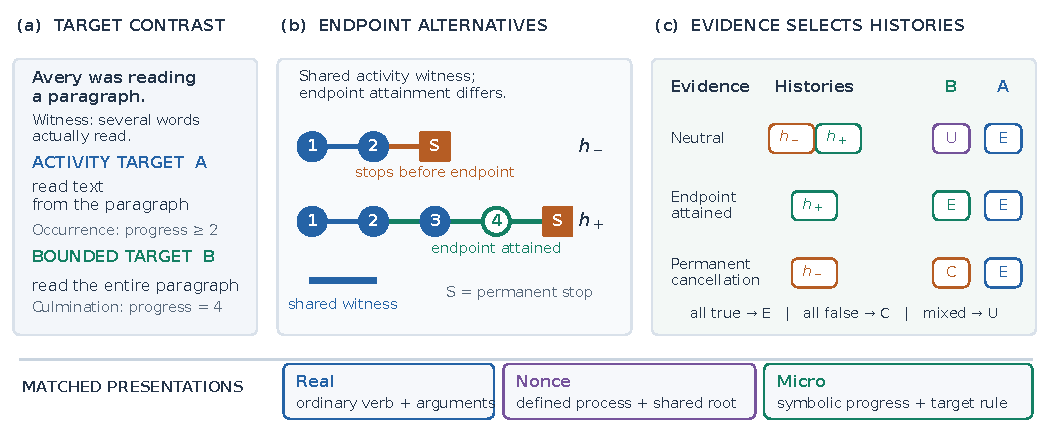
\includegraphics[width=\textwidth]{method_schematic.pdf}
\caption{Compatible-history evaluation. The reading example preserves the verb and episode while changing the target's extent. Both histories contain sufficient activity; only $h_+$ attains the endpoint. Evidence retains both histories, $h_+$, or $h_-$, yielding unknown, entailed, or contradicted for the bounded target while occurrence remains entailed. Real, Nonce and Micro render these same target truth alternatives. This is the gold-label construction, not an empirical frequency model.}
\label{fig:method}
\end{figure*}

\begin{table}[t]
\centering
\caption{Normative predictions, identical across the three matched presentations. These are theory-derived labels, not observed model accuracies.}
\label{tab:theory}
\setlength{\tabcolsep}{3pt}
\begin{tabular}{lccc}
\toprule
Evidence & \shortstack{Bounded\\target} & \shortstack{Activity\\target} & $q(B)-q(A)$\\
\midrule
Neutral & $U$ & $E$ & $[-1,0]$\\
Endpoint attained & $E$ & $E$ & $0$\\
Permanent cancellation & $C$ & $E$ & $-1$\\
\bottomrule
\end{tabular}
\end{table}

The probability columns presuppose a coherent target-truth assessment accepting the premise. A neutral bounded target has no theory-specified point probability. A strict negative neutral contrast requires a nondegenerate endpoint belief; logic gives only the weak inequality. A highly probable unknown target remains unknown as a categorical entailment judgment. No threshold maps the elicited score into a label.

\subsection{Families, Gold and Splits}
A seeded generator allocates 120 main families and 40 disjoint pilot families over 12 real lemmas and three manipulation strata. Each main lemma has ten scenario realizations. Lexical blocks, rather than individual renderings, determine the outer resampling unit.

Each family crosses three presentations, bounded/activity targets and neutral/supportive/cancelling evidence, producing 18 items. Gold comprises 12 entailed, three contradicted and three unknown items per family. We preserve this semantic imbalance and report macro-label and cell accuracy rather than forcing equal labels by changing targets. Original and generated pairs undergo exact/normalized overlap checks. Automatic checks verify allocation, shared lemmas and nonce forms, process predicates and the truth matrix. Gold never comes from model responses.

The agent, underlying theme or path, and episode horizon are matched within a pair. A bounded theme is the entire stipulated portion or text, or a marked path goal. The activity counterpart requires sufficient witnessed processing. Quantity items exclude additional target quantities; cancellation excludes endpoint attainment and later continuation within the same episode. The oracle determines all gold labels from the encoded histories and target predicates; automatic validation checks all 5,744 frozen item variants and controls. These labels are reference judgments for the specified interpretation. The two-stage witness and fixed episode horizon are explicit task assumptions, as are exclusion of surplus targets and of resumption after cancellation.

\begin{table}[t]
\centering
\caption{VP excerpts from frozen Real targets (F001, F057 and F141). The full hypotheses retain the same agent, episode and reporting horizon.}
\label{tab:vp_examples}
\setlength{\tabcolsep}{3pt}
\begin{tabular}{@{}l>{\raggedright\arraybackslash}p{.40\columnwidth}>{\raggedright\arraybackslash}p{.34\columnwidth}@{}}
\toprule
Verb & Bounded argument & Activity argument\\
\midrule
drink & exactly one measured glass of water & water\\
walk & to the marked far end of the corridor & along the corridor\\
read & the entire specified paragraph & text from the specified paragraph\\
\bottomrule
\end{tabular}
\end{table}

Matching preserves the underlying episode and endpoint truth alternatives, rather than making complete premises differ by a single word. Bounded Real items additionally exclude surplus targets; their outcome evidence names the required quantity, goal or coverage. Activity evidence states witnessed occurrence and duration. Outcome wording states the evidence required by each target, so the paired comparison evaluates full VP-and-evidence packages. Endpoint and cancellation conditions explicitly supply decisive facts; neutral conditions preserve unresolved endpoints.

\subsection{Presentations and Intended Priors}
Real uses ordinary verbs and arguments. Nonce defines a neutral process and shares its predicate root within the bounded/activity pair. Micro states symbolic progress and target rules. All three preserve the family-level endpoint truth alternatives, while differing in lexical associations, definition burden, length and notation. A Real-definition control tests an additional presentation with definitions supplied for ordinary predicates. Nonce forms pass a retained dictionary-noncollision audit.

A separate Real-bounded module crosses two intended burden levels with three contexts over 40 main families (240 items per system). Smaller portions, shorter texts and nearer goals motivate a predicted neutral completion-score increase. The cues specify intended processing burden; no prior distribution is assumed. Explicit endpoint or cancellation evidence fixes the logical label at either burden level. This module is exploratory, with no independent prior ratings.

\subsection{Models and Collection}
Six named systems are fixed before main core outcomes: Qwen3 at 8B, 14B and 32B~\cite{qwen2025}; Llama 3.1 8B Instruct~\cite{llama2024}; Ministral 8B 2512~\cite{ministral2025}; and Gemma 3 12B IT~\cite{gemma2025}. A 30-family core and 20-family intended-prior subset is reserved for DeepSeek-V3.2 stress evaluation~\cite{deepseek2025}. Stress comparisons restrict every system to the same families; DeepSeek is analyzed separately from the dense Qwen size comparison.

OpenRouter providers are fixed: Alibaba for Qwen8, Groq for Llama8, Mistral for Ministral8, and DeepInfra BF16/FP8/FP4 endpoints for Gemma, larger Qwen and DeepSeek respectively. Qwen dense parameter counts are 8.2, 14.8 and 32.8 billion. Within-Qwen comparisons report size associations under these provider and precision settings.

Requests use temperature zero, top-$p$ one, a 256-token output budget, no tools and no requested reasoning trace. Explicit gateway disable controls and the Qwen-supported \texttt{/no\_think} switch address supplier-specific hidden reasoning. Usage metadata, including residual wrapper tokens, remains recorded. The Qwen switch is applied uniformly across its three sizes and is a disclosed adaptation of the original zero-shot prompt. Non-Qwen original prompt bodies are unchanged. This is a contemporary protocol adaptation rather than exact reproduction of historical models.

Generated tasks request a short JSON judgment and subjective hypothesis probability. Label-only controls omit the latter. Successful outputs, including parse errors, are never retried. Only failed transport requests may be resumed. Full request hashes include messages, model, supplier and decoding; exact equivalents reuse the same response and are not independent stochastic replicates. All planned analysis cells remain represented, including missing outcomes.

\subsection{Pilot, Freeze and Robustness}
The disjoint two-system pilot supplies 1,600 valid responses: 720 core, 60 prior and 20 label controls per system. A 40-call schema check removes a redundant probability field. Both versions are retained. Pilot event/prior outcomes are excluded from main estimates; generic controls with identical payloads are cached, including 20 Llama controls. A timestamped local freeze precedes main core collection.

The seeded 24-family robustness subset crosses presentation, target type and neutral/cancelling evidence (288 matched cells per system). Paired variants change label order, renderer, names, output schema, natural guidance or structural guidance. The Real-definition variant changes 96 Real cells per system. Post-freeze participle-repair controls preserve original stimuli and results while assessing the known wording defects; their descriptive outcomes appear in Section~\ref{sec:robustness}.

\subsection{Metrics and Statistics}
Accuracy uses all planned cells; macro accuracy averages the three gold-label recalls. Cell diagnostics separate unresolved bounded endpoints from witnessed activity. Elicited $q$ is subjective target-truth probability, distinct from directly measured language-model string probability~\cite{hu2023}. Compositional sensitivity, $q(B)-q(A)$, measures the target-type score gap; categorical judgments independently test the all-history criterion. Thus a probable unknown outcome stays unknown, and a negative score gap can accompany a contradiction error.

Five prespecified contrasts per main model form one 30-test Holm family~\cite{holm1979}: Real neutral compositional sensitivity, its Real--Nonce and Real--Micro differences, Real bounded cancellation-minus-neutral $q$, and structural-rule accuracy gain. Marginal 95\% intervals use 10,000 seeded bootstrap draws~\cite{efron1979}, resampling verbs and then families within verbs. Exact sign flips over the 12 lexical blocks assume exchangeable block-effect signs under the null. Rule gains count failed outputs as incorrect; probability contrasts use complete pairs and report adverse missing-score bounds. The retained pool is complete. Family-only intervals are descriptive sensitivity checks.

Secondary contrasts receive BH adjustment~\cite{bh1995} within the named complete families; these are exploratory adjusted $p$-values. The prespecified lme4 mixed-effects correctness and raw-$q$ fits~\cite{bates2015} encounter separation or singularity in the core analyses; clustered contrasts provide the inferential results. All 32 fit attempts and fallback diagnostics are retained in the supplement, including the single usable exploratory prior fit.

\subsection{Reproducibility}
The anonymous package contains generated stimuli, unchanged original gold, response/attempt ledgers, all 30 primary and 380 secondary diagnostics, model-fit diagnostics, source-backed figures and offline scripts. Independent extraction reproduces the statistical outputs exactly, and disposable stimulus replay is byte-identical. Collection uses a local precollection freeze rather than external preregistration. Known returned API charges total \$0.9224; the conservative ledger, including unavailable-charge reserves, totals \$2.0425.\footnote{Research implementation: Codex assisted study-design refinement, generator and analysis implementation, literature auditing, experimental orchestration, result checks and figure production. Gold is computed by the explicit history rules; empirical outcomes are recorded API responses.}

\section{Results}
\subsection{Evaluation Coverage and Label Controls}
The six-system suite contains 28,104 planned cells and 27,984 unique payloads, including 35 cached generic controls and 120 equivalent planned cells. All formal responses are valid; transport attempts remain recorded separately. DeepSeek contributes 660 stress outcomes. The wording control covers 518 paired formal cells, including the initial 180 corrections.

Every system solves the generic entailed and contradicted controls (20/20 each); five solve all generic unknown controls. Qwen8 scores 0/20 on generic unknowns but 120/120 on Micro unknowns. This contrast identifies presentation-dependent label use. Event-specific unknown errors also persist in systems that solve the generic controls.

\begin{table*}[t]
\centering
\caption{Completed main core results (percent). Each presentation has 720 items per system: 480 entailed, 120 contradicted and 120 unknown. Acc. uses all planned cells; macro averages the three label recalls; U is unknown recall. The final column is a separate generic unknown-label control, including the disclosed cached controls. }
\label{tab:core_results}
\setlength{\tabcolsep}{4pt}
\begin{tabular}{lrrrrrrrrrr}
\toprule
 & \multicolumn{3}{c}{Real} & \multicolumn{3}{c}{Nonce} & \multicolumn{3}{c}{Micro} & Generic U\\
System & Acc. & Macro & U & Acc. & Macro & U & Acc. & Macro & U & Correct\\
\midrule
Qwen8 & 91.9 & 83.9 & 65.0 & 59.2 & 54.6 & 0.0 & 100.0 & 100.0 & 100.0 & 0/20 \\
Llama8 & 82.4 & 64.7 & 15.8 & 85.3 & 70.6 & 15.0 & 89.4 & 78.9 & 36.7 & 20/20 \\
Ministral8 & 58.3 & 67.7 & 79.2 & 73.5 & 86.7 & 100.0 & 66.7 & 83.3 & 100.0 & 20/20 \\
Gemma12 & 92.2 & 84.4 & 54.2 & 92.1 & 84.2 & 52.5 & 100.0 & 100.0 & 100.0 & 20/20 \\
Qwen14 & 94.9 & 89.7 & 70.0 & 63.5 & 57.2 & 1.7 & 86.2 & 93.1 & 100.0 & 20/20 \\
Qwen32 & 94.7 & 89.4 & 68.3 & 86.5 & 92.6 & 97.5 & 100.0 & 100.0 & 100.0 & 20/20 \\
\bottomrule
\end{tabular}
\end{table*}

\subsection{Composition, Presentation and Categorical Errors}
\begin{figure*}[t]
\centering
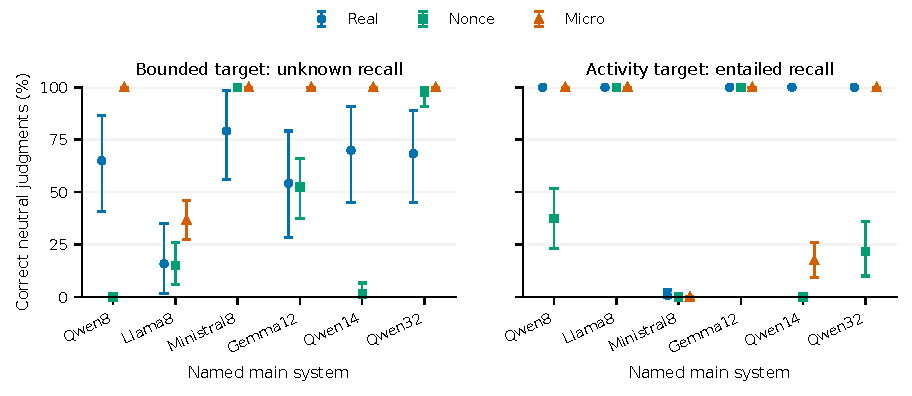
\includegraphics[width=\textwidth]{main_category_accuracy.pdf}
\caption{Neutral categorical diagnostics: unresolved endpoint versus witnessed occurrence. Each point retains 120 planned families; missing/invalid labels count incorrect. Marginal 95\% intervals use 10,000 verb-then-family bootstrap draws over 12 lexical blocks. Intervals reflect lexical/family resampling. All six systems and three presentations are shown.}
\label{fig:category}
\end{figure*}
Table~\ref{tab:core_results} shows that aggregate accuracy can conceal label-specific failure. Figure~\ref{fig:category} separates neutral endpoint uncertainty from witnessed activity occurrence. Real accuracy exceeds 91\% for four systems, while their unknown recall ranges from 54.2\% to 70.0\%. Llama8 reaches 82.4\% Real accuracy but only 15.8\% unknown recall. The majority-label proportion is 66.7\%, making macro-label and cell diagnostics necessary.

Nonce substitution does not uniformly improve reasoning. Qwen8 falls from 91.9\% Real accuracy to 59.2\% Nonce accuracy, and Qwen14 from 94.9\% to 63.5\%. Their neutral Nonce activity accuracy is respectively 37.5\% and 0\%, despite that target's explicit occurrence witness. Qwen32 also answers only 21.7\% of neutral Nonce activity targets correctly. These are occurrence errors on witnessed activity. Qwen8 calls every neutral Nonce bounded target contradicted; Qwen14 does so on 118/120 items. The dominant bounded-target error is therefore contradiction, which a completion-entailment account misses.

Micro yields perfect core accuracy for Qwen8, Gemma12 and Qwen32. It does not provide universal recovery: Llama8 reaches 89.4\%, Qwen14 86.2\%, and Ministral8 66.7\%. Ministral8 correctly identifies every Micro unknown and contradicted item but only half of the entailed items, giving 83.3\% macro accuracy. It fails every neutral Micro activity target. Qwen14 answers 17.5\% of that same cell correctly. The explicit process presentation can therefore localize failures rather than merely produce a higher total score.

All six Real neutral compositional-sensitivity point estimates are negative, ranging from $-0.504$ to $-0.248$. A negative score difference is insufficient evidence of correct categorical inference. Ministral8 has zero mean neutral Nonce and Micro contrast while failing their occurrence targets; Qwen14 has negative neutral Nonce sensitivity despite failing every neutral activity judgment. The score and categorical outcomes must be interpreted jointly.

Explicit cancellation establishes the negative operational label: Real bounded cancellation accuracy is 100\% for Qwen32, 99.2\% for Gemma12 and Qwen14, 86.7\% for Qwen8, 78.3\% for Llama8, and 75.0\% for Ministral8. All systems reach 100\% in the corresponding Micro cell. The Real estimates retain the original wording; Section~
ef{sec:robustness} reports the paired correction check.

\subsection{Prespecified Clustered Contrasts}
\begin{table*}[t]
\centering
\caption{All 30 prespecified contrasts. Each cell gives estimate, marginal lexical/family bootstrap 95\% CI, and Holm-adjusted $p$ across the complete 30-test family. The first four columns are q differences over 120 complete paired families; the rule column is percentage-point accuracy change over 24 complete families with 12 matched cells each. Exact block sign flips use the retained lexical blocks. Marginal intervals and adjusted tests have different multiplicity scopes. All planned probability contrasts have complete scores, so adverse bounds equal the point estimate.}
\label{tab:primary_results}
\setlength{\tabcolsep}{5pt}
\begin{tabular}{lrrrrr}
\toprule
System & Real CS & Real--Nonce CS & Real--Micro CS & Cancel--neutral q & Structural rule\\
\midrule
Qwen8 & \shortstack{$-0.344$\\$[-0.457,-0.220]$\\$0.043$} & \shortstack{$0.372$\\$[0.235,0.521]$\\$0.015$} & \shortstack{$0.156$\\$[0.043,0.280]$\\$0.279$} & \shortstack{$-0.485$\\$[-0.585,-0.381]$\\$0.015$} & \shortstack{$-0.69$\\$[-2.63,1.09]$\\$1.000$} \\[3pt]
Llama8 & \shortstack{$-0.504$\\$[-0.713,-0.300]$\\$0.065$} & \shortstack{$-0.016$\\$[-0.223,0.186]$\\$1.000$} & \shortstack{$-0.321$\\$[-0.537,-0.108]$\\$0.240$} & \shortstack{$-0.279$\\$[-0.421,-0.138]$\\$0.109$} & \shortstack{$3.82$\\$[0.83,6.67]$\\$0.279$} \\[3pt]
Ministral8 & \shortstack{$-0.248$\\$[-0.361,-0.140]$\\$0.065$} & \shortstack{$-0.248$\\$[-0.361,-0.140]$\\$0.065$} & \shortstack{$-0.248$\\$[-0.361,-0.140]$\\$0.065$} & \shortstack{$-0.446$\\$[-0.602,-0.277]$\\$0.043$} & \shortstack{$3.12$\\$[0.00,6.79]$\\$1.000$} \\[3pt]
Gemma12 & \shortstack{$-0.274$\\$[-0.417,-0.141]$\\$0.109$} & \shortstack{$0.421$\\$[0.290,0.541]$\\$0.015$} & \shortstack{$0.017$\\$[-0.127,0.149]$\\$1.000$} & \shortstack{$-0.665$\\$[-0.805,-0.511]$\\$0.015$} & \shortstack{$-2.78$\\$[-5.16,-0.32]$\\$0.703$} \\[3pt]
Qwen14 & \shortstack{$-0.315$\\$[-0.415,-0.202]$\\$0.065$} & \shortstack{$0.233$\\$[0.130,0.348]$\\$0.015$} & \shortstack{$-0.062$\\$[-0.175,0.061]$\\$1.000$} & \shortstack{$-0.677$\\$[-0.784,-0.582]$\\$0.015$} & \shortstack{$0.00$\\$[-1.92,2.08]$\\$1.000$} \\[3pt]
Qwen32 & \shortstack{$-0.308$\\$[-0.410,-0.198]$\\$0.043$} & \shortstack{$-0.074$\\$[-0.200,0.067]$\\$1.000$} & \shortstack{$0.277$\\$[0.169,0.392]$\\$0.015$} & \shortstack{$-0.692$\\$[-0.802,-0.590]$\\$0.015$} & \shortstack{$1.74$\\$[-0.31,3.62]$\\$1.000$} \\[3pt]
\bottomrule
\end{tabular}
\end{table*}

Table~\ref{tab:primary_results} centralizes the uncertainty and multiplicity reporting. Real neutral sensitivity is negative in all six systems; Qwen8 and Qwen32 pass Holm correction. Positive Real--Nonce differences pass for Qwen8, Gemma12 and Qwen14: their Nonce score gaps are more negative despite the categorical failures above. Qwen32 also has a positive corrected Real--Micro difference. These results directly show why the direction of a score contrast and correctness of event inference must be evaluated separately.

Cancellation lowers bounded Real scores in all systems, with five corrected contrasts passing. Structural-rule gains range from $-2.78$ to $+3.82$ percentage points; none passes the complete Holm family. The evidence supports contextual override but no corrected accuracy improvement from structural guidance in this setup. Marginal intervals and adjusted tests have their respective scopes stated in the table. Full family-only interval and mixed-fit diagnostics are supplied with the results.

\subsection{Contemporary Original-Benchmark Replication}
\begin{table*}[t]
\centering
\caption{Contemporary ImperfectiveNLI replication (percent), with unchanged original gold. Acc. is original-gold accuracy. TBR is the true-response rate in the named group, whose original gold is false (A) or unknown (C). Full: 400 items (A/C each 100); published VSS: 303 (A 49, C 58); explicit noncompletion: 24 Group A items. Different subsets are distinct diagnostics, not paired estimates of an improvement. All responses parse successfully.}
\label{tab:replication_results}
\setlength{\tabcolsep}{5pt}
\begin{tabular}{lrrrrrrrr}
\toprule
 & \multicolumn{3}{c}{Full original} & \multicolumn{3}{c}{Published VSS} & \multicolumn{2}{c}{A explicit}\\
System & Acc. & TBR A & TBR C & Acc. & TBR A & TBR C & Acc. & TBR A\\
\midrule
Qwen8 & 57.5 & 56.0 & 84.0 & 73.3 & 44.9 & 75.9 & 29.2 & 41.7 \\
Llama8 & 53.2 & 55.0 & 94.0 & 67.3 & 38.8 & 93.1 & 45.8 & 33.3 \\
Ministral8 & 58.5 & 33.0 & 55.0 & 70.6 & 18.4 & 43.1 & 33.3 & 16.7 \\
Gemma12 & 57.5 & 51.0 & 81.0 & 72.6 & 40.8 & 70.7 & 29.2 & 50.0 \\
Qwen14 & 68.0 & 29.0 & 50.0 & 80.2 & 14.3 & 43.1 & 54.2 & 8.3 \\
Qwen32 & 63.2 & 49.0 & 98.0 & 76.9 & 28.6 & 96.6 & 66.7 & 33.3 \\
\bottomrule
\end{tabular}
\end{table*}
The unchanged 400-item benchmark yields 53.2--68.0\% accuracy; the published 303-item filter yields 67.3--80.2\% on a differently composed pool (Table~\ref{tab:replication_results}). Group C true-response rates remain 43.1--96.6\% after filtering. In the 24 Group A items with explicit noncompletion, true-response rates remain 8.3--50.0\%. Thus the contemporary response pattern includes errors under explicit negative evidence as well as disputed original interpretations.

We retain distinct denominators and unchanged gold for the full pool, the published filter, and the subset with explicit noncompletion. Llama8 and Qwen32 have high Group C true rates despite correct generic unknown controls. These observations motivate separating task-specific uncertainty errors from global label use, as the compatible-history benchmark does. The replication uses current endpoints and the disclosed Qwen prompt adaptation; it is a contemporary diagnostic alongside the original benchmark.

\subsection{Intervention and Robustness Tests}
\label{sec:robustness}
Natural guidance changes matched accuracy by $-3.8$ to $+5.6$ points. In the complete secondary intervention family, it improves Llama8 by 5.56 points (BH $p=0.020$) and reduces Gemma12 by 3.82 points ($p=0.049$). Together with the primary structural-rule results, these opposite directions establish system-dependent intervention behavior. Held-out rendering changes model accuracy by $-9.0$ to $+11.5$ points; the Real-definition variant changes its 96 affected Real cells by zero to $+7.3$ points. All paired variants and denominators are retained in the supplement.

Neutral burden-cue score shifts are positive in all six main systems ($0.030$--$0.140$), but none of the complete 21 prior-context contrasts passes BH correction (minimum adjusted $p=0.185$). The evidence is inconclusive for the predicted cue effect. Within Qwen, Micro accuracy is 100\%, 86.2\% and 100\% at 8.2, 14.8 and 32.8 billion parameters. Performance is nonmonotonic under the evaluated providers and precisions.

A post-freeze audit identifies incorrect passive participles for drink, eat and write in 30 Real bounded cancellation core items. The complete paired correction covers all inherited formal defects: 83 cells per main system and 20 stress cells (518 pairs). Twelve labels change, including one improved Ministral core answer and one worsened Gemma core answer; all 20 affected DeepSeek labels remain unchanged. Original primary outcomes are preserved. The correction is a later descriptive check, with service/order variation; it adds no inferential tests.

\subsection{Matched Strong-Model Stress Test}
Every system is compared on the same 30 core families (540 items, 180 per presentation). DeepSeek reaches 90.0\% Real, 98.3\% Nonce and 100\% Micro accuracy, with macro accuracies of 80.0\%, 96.7\% and 100\%. The corresponding matched main-system accuracy ranges are 57.8--93.9\%, 57.8--93.9\% and 66.7--100\%. Three main systems also solve every Micro item on this subset.

DeepSeek's Real unknown recall is 46.7\% (14/30), whereas its Nonce unknown recall is 90.0\% (27/30). Its Real entailed and contradicted recalls are 100\% and 93.3\%. Strong Nonce/Micro performance thus coexists with unresolved-endpoint errors in ordinary language. This matched stress result confirms the ordinary-language uncertainty failure alongside successful explicit-process inference.



\subsection{Surface Recoverability and Rendering}
The fixed word-unigram full-text baseline trained on disjoint pilot gold reaches 95.4\% main core accuracy and 90.7\% macro accuracy. Hypothesis-only and majority baselines both reach 66.7\% accuracy, with macro accuracies of 35.7\% and 33.3\%. Strong full-text performance establishes surface recoverability in this controlled construction set. On the same 24-family, 288-item subset, full-text baseline accuracy drops from 92.7\% with the original renderer to 76.0\% with the held-out renderer, a paired 16.7-point decrease. The baseline receives labeled pilot training. Its strong in-template fit and renderer drop establish that surface cues recover much of the controlled set while depending on its wording.

\section{Discussion}
Compatible-history evaluation turns an aggregate completion judgment into three inspectable tests: occurrence, culmination and uncertainty. Its empirical value is visible in the Nonce results. An unresolved bounded target can receive a low score and an incorrect contradiction label, while its witnessed activity counterpart is also rejected. A single negative completion contrast hides both failures. Category-level evaluation supplies the missing distinction.

Presentation comparisons distinguish rule application from language interpretation. Qwen8, Gemma12 and Qwen32 each solve the full Micro core. DeepSeek reproduces that ceiling on the matched stress subset while retaining Real unknown errors. Explicit rules therefore provide a useful reference condition for localizing interpretation difficulty. Defined predicates create additional occurrence failures, showing that lexical replacement changes the evaluation task as well as lexical associations.

The intervention and surface diagnostics explain how to use this benchmark. Structural guidance supplies no accuracy gain passing the primary correction; natural guidance helps one system and harms another in secondary tests. The supervised baseline fits the original templates well but loses accuracy on the new renderer. This supports using the benchmark as a structured diagnostic with paired controls. Together these findings support reporting category profiles and presentation sensitivity alongside aggregate accuracy and subjective scores.

\balance
\section{Scope and Limitations}
The task specifies a single episode, sufficient witnessed activity and explicit endpoint truth alternatives. It evaluates adherence to those readings. The 12-lemma inventory and repeated process mechanisms delimit linguistic coverage; lexical/family resampling reflects that design. Ordinary, defined-predicate and symbolic presentations differ in information burden, so layer effects compare presentation packages. Providers, precision and training also differ across systems. Elicited scores are uncalibrated; the burden-cue analysis measures subjective shifts without independent prior ratings. Known participle defects and their complete later paired correction are reported in Section~\ref{sec:robustness}. Extending the construction inventory and testing implicit outcomes in broader discourse are natural next evaluation settings.

\section{Conclusion}
We introduce compatible-history evaluation for separating event occurrence, culmination and unresolved outcomes. The matched benchmark exposes categorical failures that aggregate accuracy and completion-score contrasts conceal. Six-system results and a matched strong-model stress test show that perfect explicit-process inference can coexist with ordinary-language uncertainty errors, while defined predicates introduce distinct occurrence and contradiction failures. This provides a reproducible method for diagnosing which event truth conditions a language model preserves across target types, evidence and presentations.



\begin{thebibliography}{99}
\bibitem{vendler1957} Zeno Vendler. 1957. Verbs and Times. \emph{The Philosophical Review} 66(2), 143--160.
\bibitem{moens1988} Marc Moens and Mark Steedman. 1988. Temporal Ontology and Temporal Reference. \emph{Computational Linguistics} 14(2), 15--28.
\bibitem{krifka1998} Manfred Krifka. 1998. The Origins of Telicity. In \emph{Events and Grammar}, Susan Rothstein (Ed.). Kluwer, 197--235.
\bibitem{ma2026} Bolei Ma and Yusuke Miyao. 2026. The Imperfective Paradox in Large Language Models. In \emph{Proceedings of ACL}, 15093--15111. \url{https://aclanthology.org/2026.acl-long.689/}
\bibitem{han2026} Kaiqiao Han and Yizhou Sun. 2026. The imperfective paradox is not necessarily in Large Language Models: A benchmark failure before a model failure. arXiv:2608.25005v1. \url{https://arxiv.org/abs/2608.25005}
\bibitem{prus2024} Katarzyna Pru\'{s}, Mark Steedman, and Adam Lopez. 2024. Human Temporal Inferences Go Beyond Aspectual Class. In \emph{Proceedings of EACL}, 1913--1923. \url{https://aclanthology.org/2024.eacl-long.115/}
\bibitem{prus2025} Katarzyna Pru\'{s}, Mark Steedman, and Adam Lopez. 2025. World Knowledge Resolves Some Aspectual Ambiguity. In \emph{Findings of ACL}, 13207--13220. \url{https://aclanthology.org/2025.findings-acl.683/}
\bibitem{core2025} Sai P Vallurupalli and Francis Ferraro. 2025. CoRE: Condition-based Reasoning for Identifying Outcome Variance in Complex Events. In \emph{Findings of ACL}, 19381--19401. \url{https://aclanthology.org/2025.findings-acl.992/}
\bibitem{cxmp2026} Miyu Oba and Saku Sugawara. 2026. CxMP: A Linguistic Minimal-Pair Benchmark for Evaluating Constructional Understanding in Language Models. In \emph{Proceedings of ACL}, 45949--45963. \url{https://aclanthology.org/2026.acl-long.2132/}
\bibitem{cogs2020} Najoung Kim and Tal Linzen. 2020. COGS: A Compositional Generalization Challenge Based on Semantic Interpretation. In \emph{Proceedings of EMNLP}, 9087--9105. \url{https://aclanthology.org/2020.emnlp-main.731/}
\bibitem{hans2019} R. Thomas McCoy, Ellie Pavlick, and Tal Linzen. 2019. Right for the Wrong Reasons: Diagnosing Syntactic Heuristics in Natural Language Inference. In \emph{Proceedings of ACL}, 3428--3448. \url{https://aclanthology.org/P19-1334/}
\bibitem{maccartney2008} Bill MacCartney and Christopher D. Manning. 2008. Modeling Semantic Containment and Exclusion in Natural Language Inference. In \emph{Proceedings of COLING}, 521--528. \url{https://aclanthology.org/C08-1066/}
\bibitem{poliak2018} Adam Poliak, Jason Naradowsky, Aparajita Haldar, Rachel Rudinger, and Benjamin Van Durme. 2018. Hypothesis Only Baselines in Natural Language Inference. In \emph{Proceedings of *SEM}, 180--191. \url{https://aclanthology.org/S18-2023/}
\bibitem{checklist2020} Marco Tulio Ribeiro, Tongshuang Wu, Carlos Guestrin, and Sameer Singh. 2020. Beyond Accuracy: Behavioral Testing of NLP Models with CheckList. In \emph{Proceedings of ACL}, 4902--4912. \url{https://aclanthology.org/2020.acl-main.442/}
\bibitem{landman1992} Fred Landman. 1992. The Progressive. \emph{Natural Language Semantics 1(1), 1--32}. \url{https://doi.org/10.1007/BF02342615}
\bibitem{proofwriter2021} Oyvind Tafjord, Bhavana Dalvi, and Peter Clark. 2021. ProofWriter: Generating Implications, Proofs, and Abductive Statements over Natural Language. \emph{Findings of ACL, 3621--3634}. \url{https://aclanthology.org/2021.findings-acl.317/}
\bibitem{timebench2024} Zheng Chu, Jingchang Chen, Qianglong Chen, Weijiang Yu, Haotian Wang, Ming Liu, and Bing Qin. 2024. TimeBench: A Comprehensive Evaluation of Temporal Reasoning Abilities in Large Language Models. \emph{Proceedings of ACL, 1204--1228}. \url{https://aclanthology.org/2024.acl-long.66/}
\bibitem{tram2024} Yuqing Wang and Yun Zhao. 2024. TRAM: Benchmarking Temporal Reasoning for Large Language Models. \emph{Findings of ACL, 6389--6415}. \url{https://aclanthology.org/2024.findings-acl.382/}
\bibitem{blimp2020} Alex Warstadt, Alicia Parrish, Haokun Liu, Anhad Mohananey, Wei Peng, Sheng-Fu Wang, and Samuel R. Bowman. 2020. BLiMP: The Benchmark of Linguistic Minimal Pairs for English. \emph{Transactions of the Association for Computational Linguistics 8, 377--392}. \url{https://aclanthology.org/2020.tacl-1.25/}
\bibitem{gururangan2018} Suchin Gururangan, Swabha Swayamdipta, Omer Levy, Roy Schwartz, Samuel R. Bowman, and Noah A. Smith. 2018. Annotation Artifacts in Natural Language Inference Data. \emph{Proceedings of NAACL-HLT, 107--112}. \url{https://aclanthology.org/N18-2017/}
\bibitem{hu2023} Jennifer Hu and Roger Levy. 2023. Prompting is not a substitute for probability measurements in large language models. \emph{Proceedings of EMNLP, 5040--5060}. \url{https://aclanthology.org/2023.emnlp-main.306/}
\bibitem{holm1979} Sture Holm. 1979. A Simple Sequentially Rejective Multiple Test Procedure. \emph{Scandinavian Journal of Statistics 6(2), 65--70}. \url{https://www.jstor.org/stable/4615733}
\bibitem{bh1995} Yoav Benjamini and Yosef Hochberg. 1995. Controlling the False Discovery Rate: A Practical and Powerful Approach to Multiple Testing. \emph{Journal of the Royal Statistical Society: Series B 57(1), 289--300}. \url{https://doi.org/10.1111/j.2517-6161.1995.tb02031.x}
\bibitem{efron1979} Bradley Efron. 1979. Bootstrap Methods: Another Look at the Jackknife. \emph{The Annals of Statistics 7(1), 1--26}. \url{https://doi.org/10.1214/aos/1176344552}
\bibitem{bates2015} Douglas Bates, Martin M\"achler, Ben Bolker, and Steve Walker. 2015. Fitting Linear Mixed-Effects Models Using lme4. \emph{Journal of Statistical Software 67(1), 1--48}. \url{https://doi.org/10.18637/jss.v067.i01}
\bibitem{salton1988} Gerard Salton and Christopher Buckley. 1988. Term-weighting approaches in automatic text retrieval. \emph{Information Processing and Management 24(5), 513--523}. \url{https://doi.org/10.1016/0306-4573(88)90021-0}
\bibitem{sklearn2011} Fabian Pedregosa et al.. 2011. Scikit-learn: Machine Learning in Python. \emph{Journal of Machine Learning Research 12, 2825--2830}. \url{https://www.jmlr.org/papers/v12/pedregosa11a.html}
\bibitem{qwen2025} An Yang et al.. 2025. Qwen3 Technical Report. \emph{arXiv:2505.09388}. \url{https://arxiv.org/abs/2505.09388}
\bibitem{llama2024} Aaron Grattafiori et al.. 2024. The Llama 3 Herd of Models. \emph{arXiv:2407.21783}. \url{https://arxiv.org/abs/2407.21783}
\bibitem{gemma2025} Gemma Team et al.. 2025. Gemma 3 Technical Report. \emph{arXiv:2503.19786}. \url{https://arxiv.org/abs/2503.19786}
\bibitem{deepseek2025} DeepSeek-AI et al.. 2025. DeepSeek-V3.2: Pushing the Frontier of Open Large Language Models. \emph{arXiv:2512.02556}. \url{https://arxiv.org/abs/2512.02556}
\bibitem{ministral2025} Mistral AI. 2025. Ministral-3-8B-Instruct-2512. \emph{Official model card}. \url{https://huggingface.co/mistralai/Ministral-3-8B-Instruct-2512}
\end{thebibliography}
\end{document}
